\subsection{Lumerical}
\label{ss:lumerical}

Lumerical FDTD Solutions es un solucionador 3D de las ecuaciones de Maxwell, 
capaz de analizar la interacción de la radiación UV, visible, IR y con estructuras complejas
 que emplean características de longitud de onda de escala. 
FDTD Solutions es capaz de tomar en cuenta de forma precisa la dispersión en un material dentro de 
intervalos de longitudes de onda, lo que permite al usuario final para calcular eficientemente la respuesta dispositivo a través de grandes rangos de ancho de banda. 

Posee un motor computacional altamente optimizado capaz de explotar sistemas de varios núcleos de computación en todo, desde computadoras portátiles hasta clusters de computación de alto rendimiento, y un framework de optimización para acelerar la generación de dispositivos nanofotónicos optimizados \cite{Lumerical_web}.

Posee las siguientes características

\begin{itemize}
\item Simulación de geometrías arbitrarias en 2D, 3D.
\item Computación Concurrente en varios equipos y cómputo paralelo en sistemas 
multicore y multiNode
\item Framework de optimización.
\item Capacidad de modelamiento de materiales con caracterísitcas dispersivas, 
de ganancia no lineal y anisotrópicos.
\item Potente lenguaje de scripts cuya sintaxis es similar a la de matlab.
\end{itemize} 

\subsubsection{Resultados}

Sobre esta plataforma, se ejecutaron las simulaciones del resonador descrito en la
sección \label{sss:rr_design} para las configuraciones de los filtros Notch y 
AddDrop. 

\paragraph{Filtro Notch}~\\

La configuración del filtro notch se realizó en 3 dimensiones. Se empleó un paralelipípedo
como el material base en Silica y la estructura básica del resonador de anillo en
Silicio que viene incluida en los componentes ópticos del software.
Para eliminar la guía del $puerto_d$, se realizó una ligera modificación
al script que general la estructura (ver apéndice \ref{ap:lum_notch}).

\begin{figure}[H]
\caption{SetUp del filtro Notch en Lumerical FDTD}
\centering
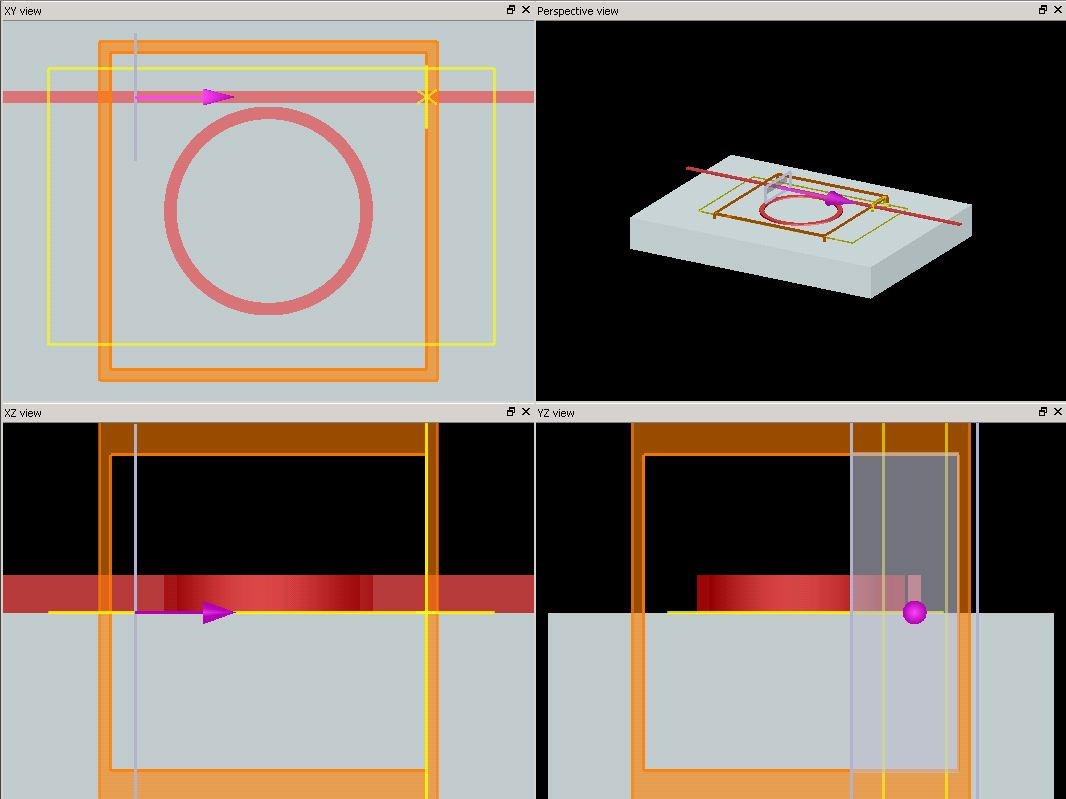
\includegraphics[width=1.0\textwidth,natwidth=1066,natheight=799]{figs/lum_setup_n.jpg}
\label{fig:lum_setup_n}
\end{figure} 

Se obtuvo el valor de la transmitancia, cuyo valor teórico está dado por la 
ecuación \ref{eq:lum_Tt}, para 500 valores de longitud de onda entre 1500 y
1600 nm como se ve en la siguiente figura:

\begin{figure}[H]
\caption{Transmitancia simulación 3D FDTD Filtro Notch}
\centering
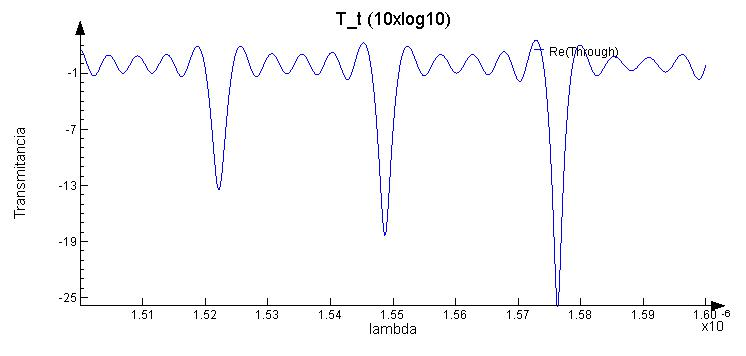
\includegraphics[width=0.8\textwidth,natwidth=605,natheight=356]{figs/lum_t_n.jpg}
\label{fig:lum_t_fdtd_n}
\end{figure} 


\paragraph{Filtro AddDrop}~\\
La configuración del filtro AddDrop se realizó de forma similar al filtro Notch 
simplemente adicionando la guía inferior sobre la que se encuentra el $puerto_d$. 

\begin{figure}[H]
\caption{SetUp del filtro AddDrop en Lumerical FDTD}
\centering
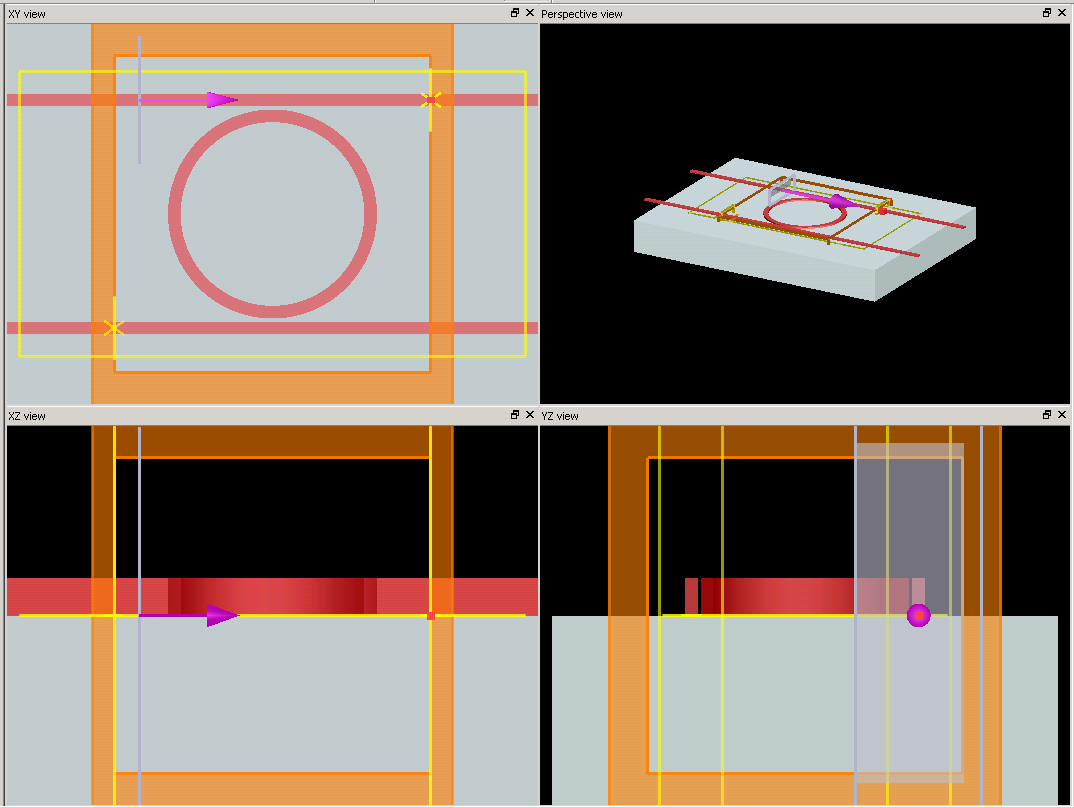
\includegraphics[width=1.0\textwidth,natwidth=1074,natheight=808]{figs/lum_setup_ad.PNG}
\label{fig:lum_setup_ad}
\end{figure} 

\begin{figure}[H]
\caption{Transmitancia en el $puerto_d$ de valores teóricos, simulación MODE y 
FDTD del Filtro AddDrop}
\centering
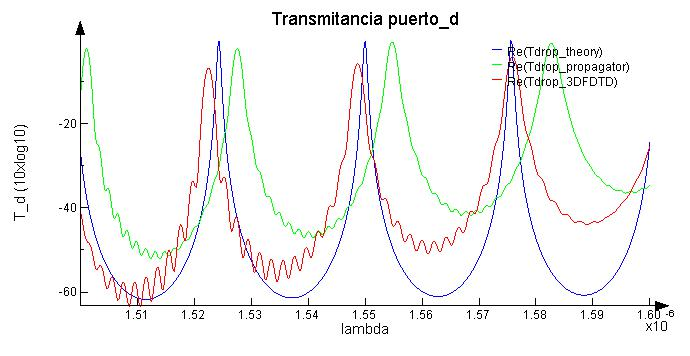
\includegraphics[width=0.8\textwidth,natwidth=593,natheight=356]{figs/lum_Td.jpg}
\label{fig:lum_td_ad}
\end{figure} 

\begin{figure}[H]
\caption{Transmitancia en el $puerto_t$ de valores teóricos, simulación MODE y 
FDTD del Filtro AddDrop}
\centering
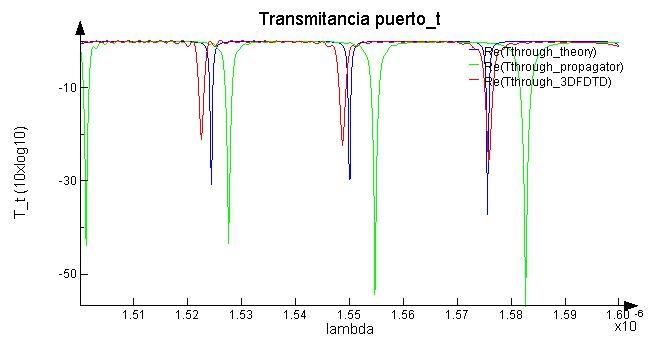
\includegraphics[width=0.8\textwidth,natwidth=632,natheight=356]{figs/lum_Tt.jpg}
\label{fig:lum_tt_ad}
\end{figure} 

\begin{figure}[H]
\caption{Transmitancia simulación 3D FDTD Filtro AddDrop}
\centering
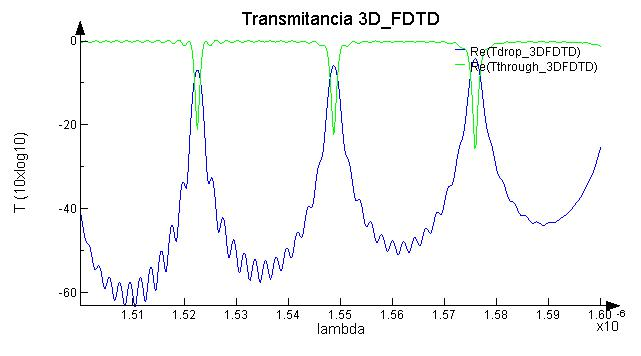
\includegraphics[width=0.8\textwidth,natwidth=598,natheight=356]{figs/lum_T_FDTD.jpg}
\label{fig:lum_t_fdtd_ad}
\end{figure} 

